\chapter{
2012: A Spatial Capture-Recapture Odyssey
}

\markboth{The End}{}
\label{chapt.final}

\vspace{0.3cm}





% XXX RS: I would move the figures so the chapter starts with text. Although the combo of the chapter title and the fisher picture is quite amusing.

\begin{figure}[h!]
\centering
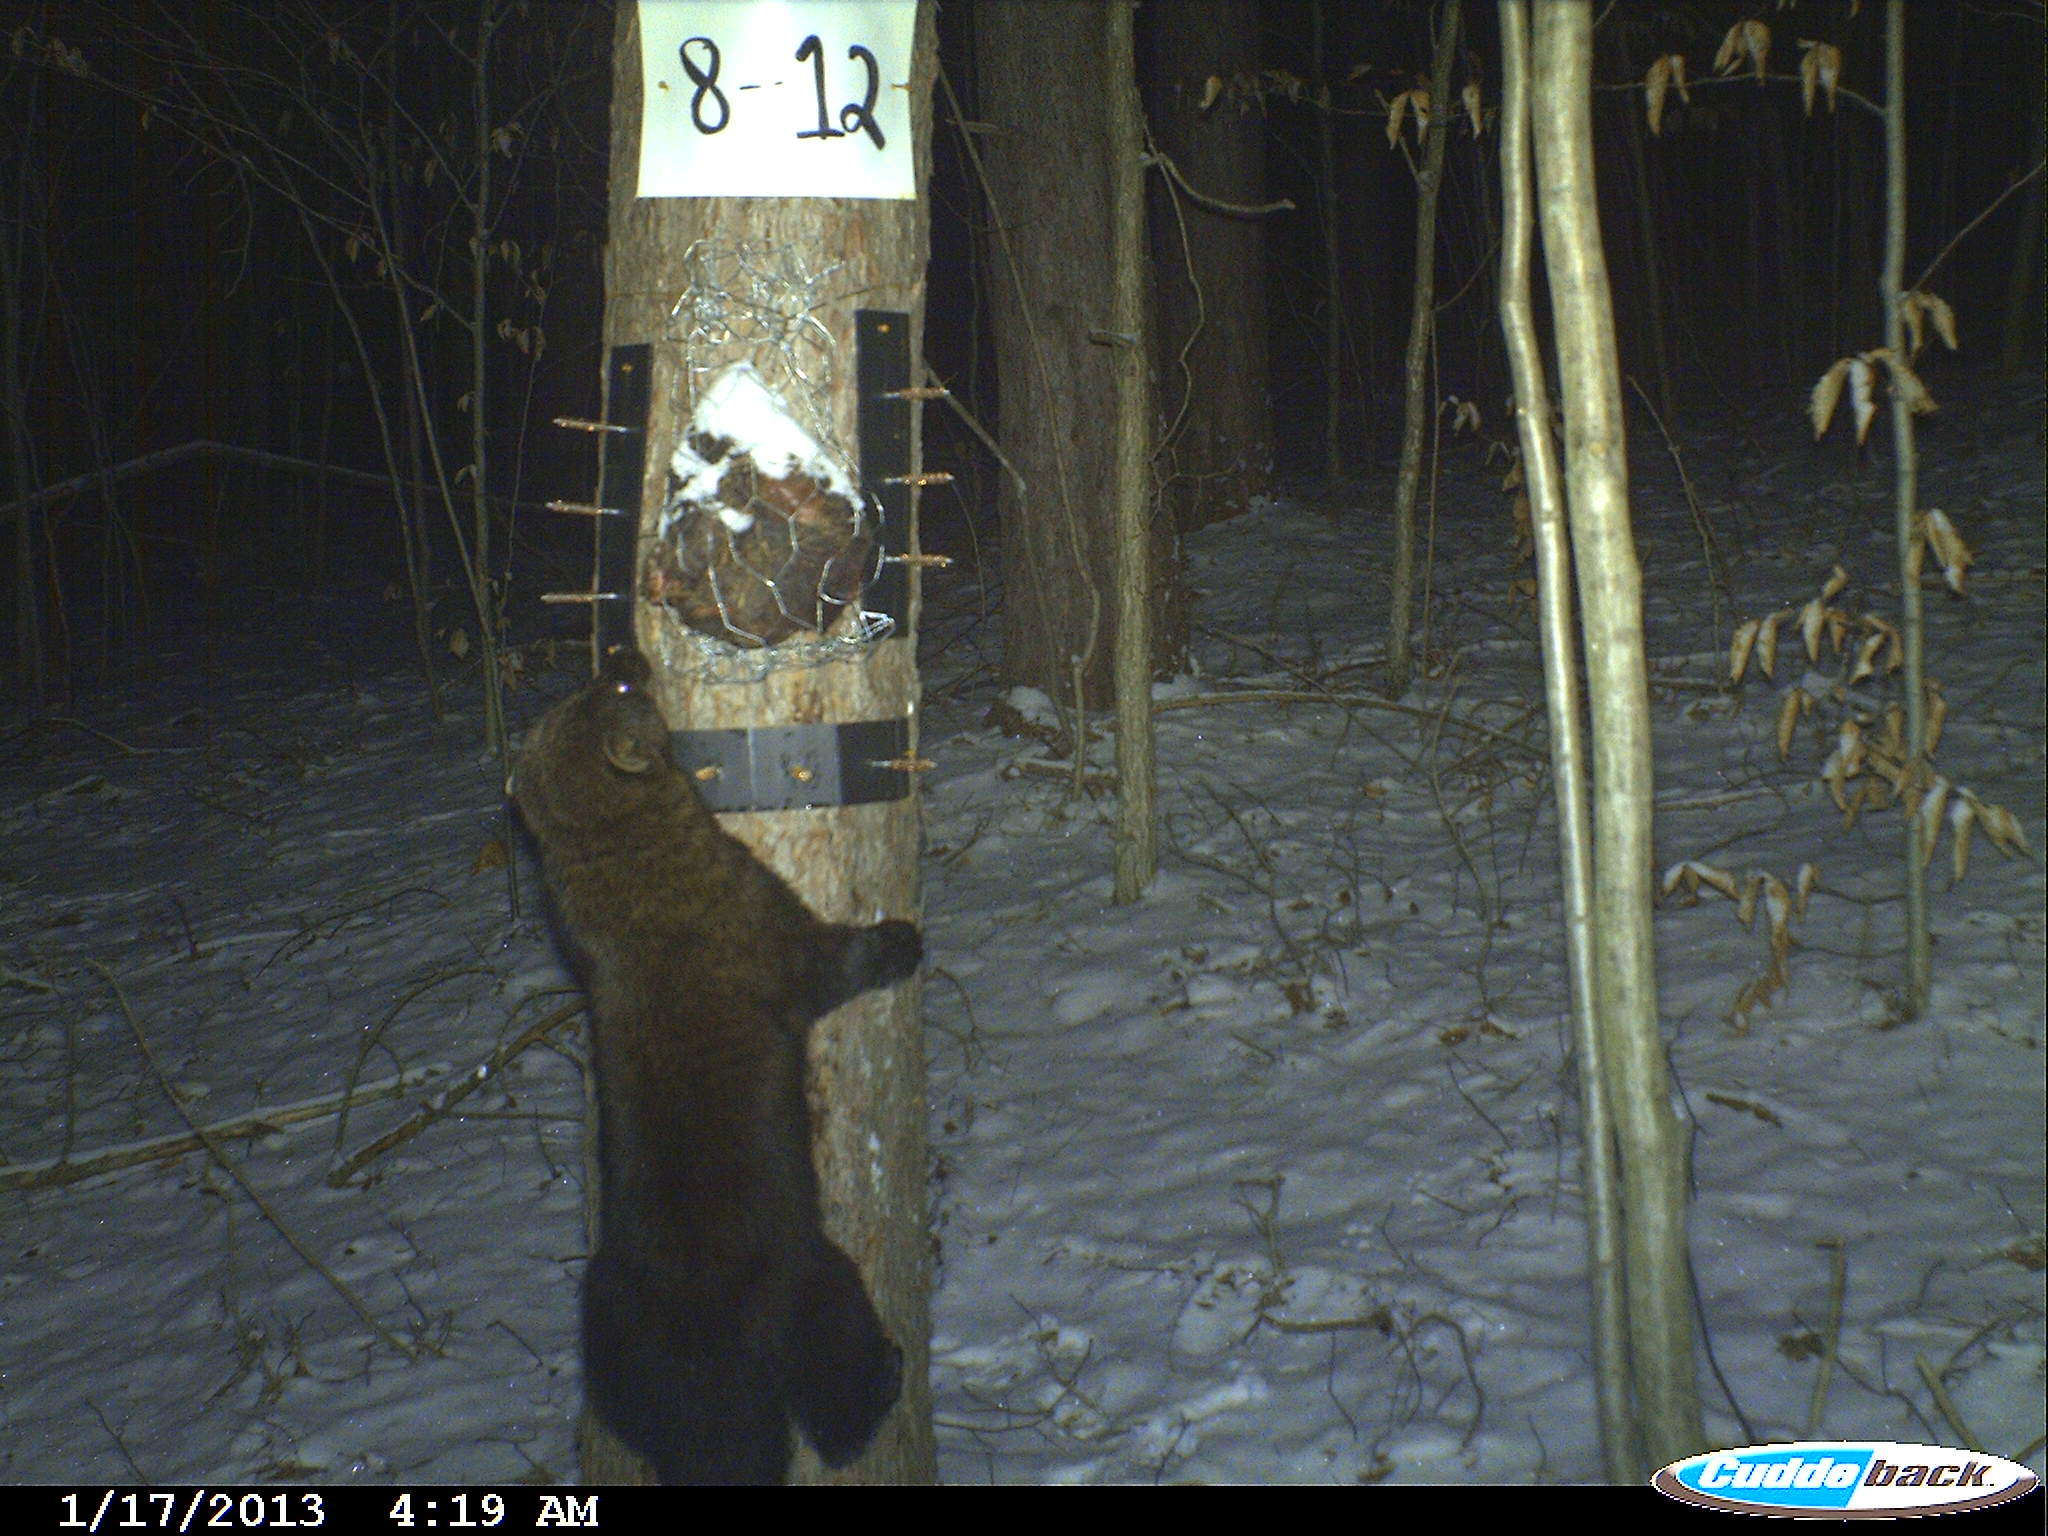
\includegraphics[width=\textwidth]{Ch20-Last/fisher.jpg}
\caption{
Fisher assaulting tree \# 8-12, outfitted with a baited hair snare.
{\it Photo credit: NYSDEC (New York State Department of Environmental Conservation),
A Fuller/NYSDEC camera trap and hair snare study of fishers in
southern NY}
}
\label{last.fig.fisher}
\end{figure}
% XX RS: Maybe change pic caption to "Fisher assaulting tree with baited hair snare \# 8-12"

\begin{figure}[h!]
\centering
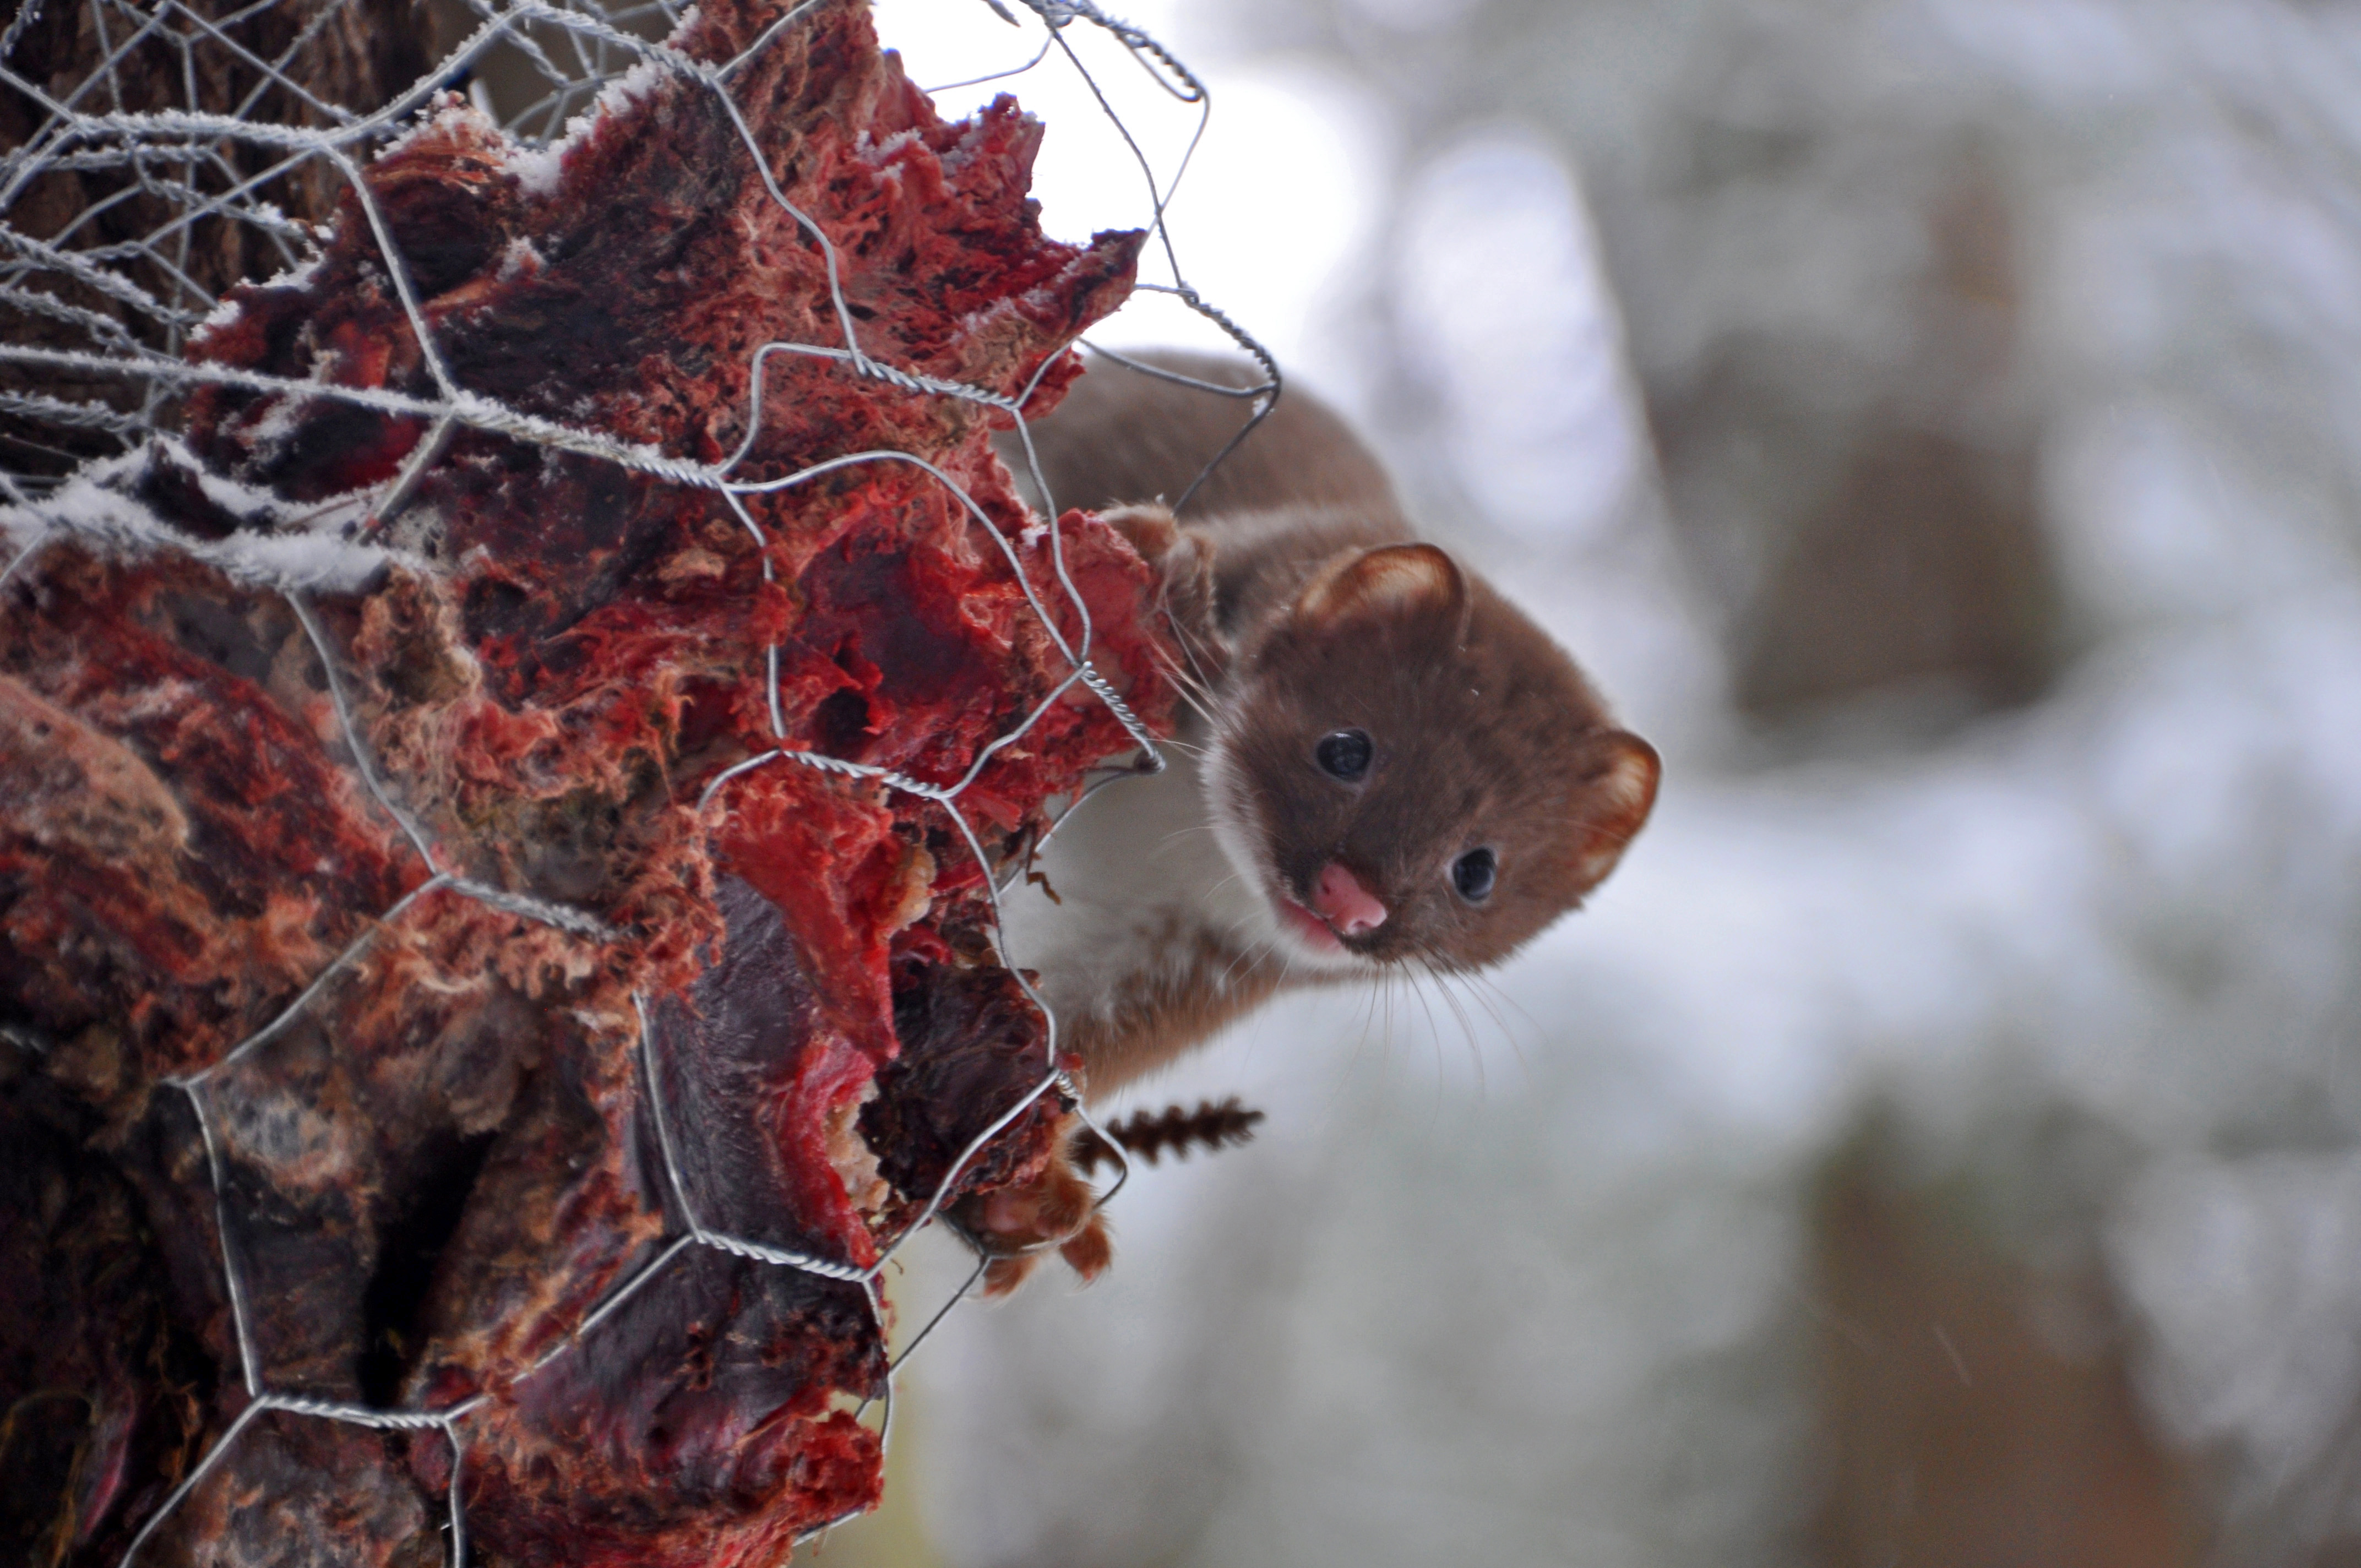
\includegraphics[width=\textwidth]{Ch20-Last/weasel.jpg}
\caption{
A long-tailed weasel taking bait on a hair snare, A. Fuller southern NY fisher study
{\it Photo credit: Marty DeLong}.
}
\label{last.fig.weasels}
\end{figure}



\begin{figure}[h!]
\centering
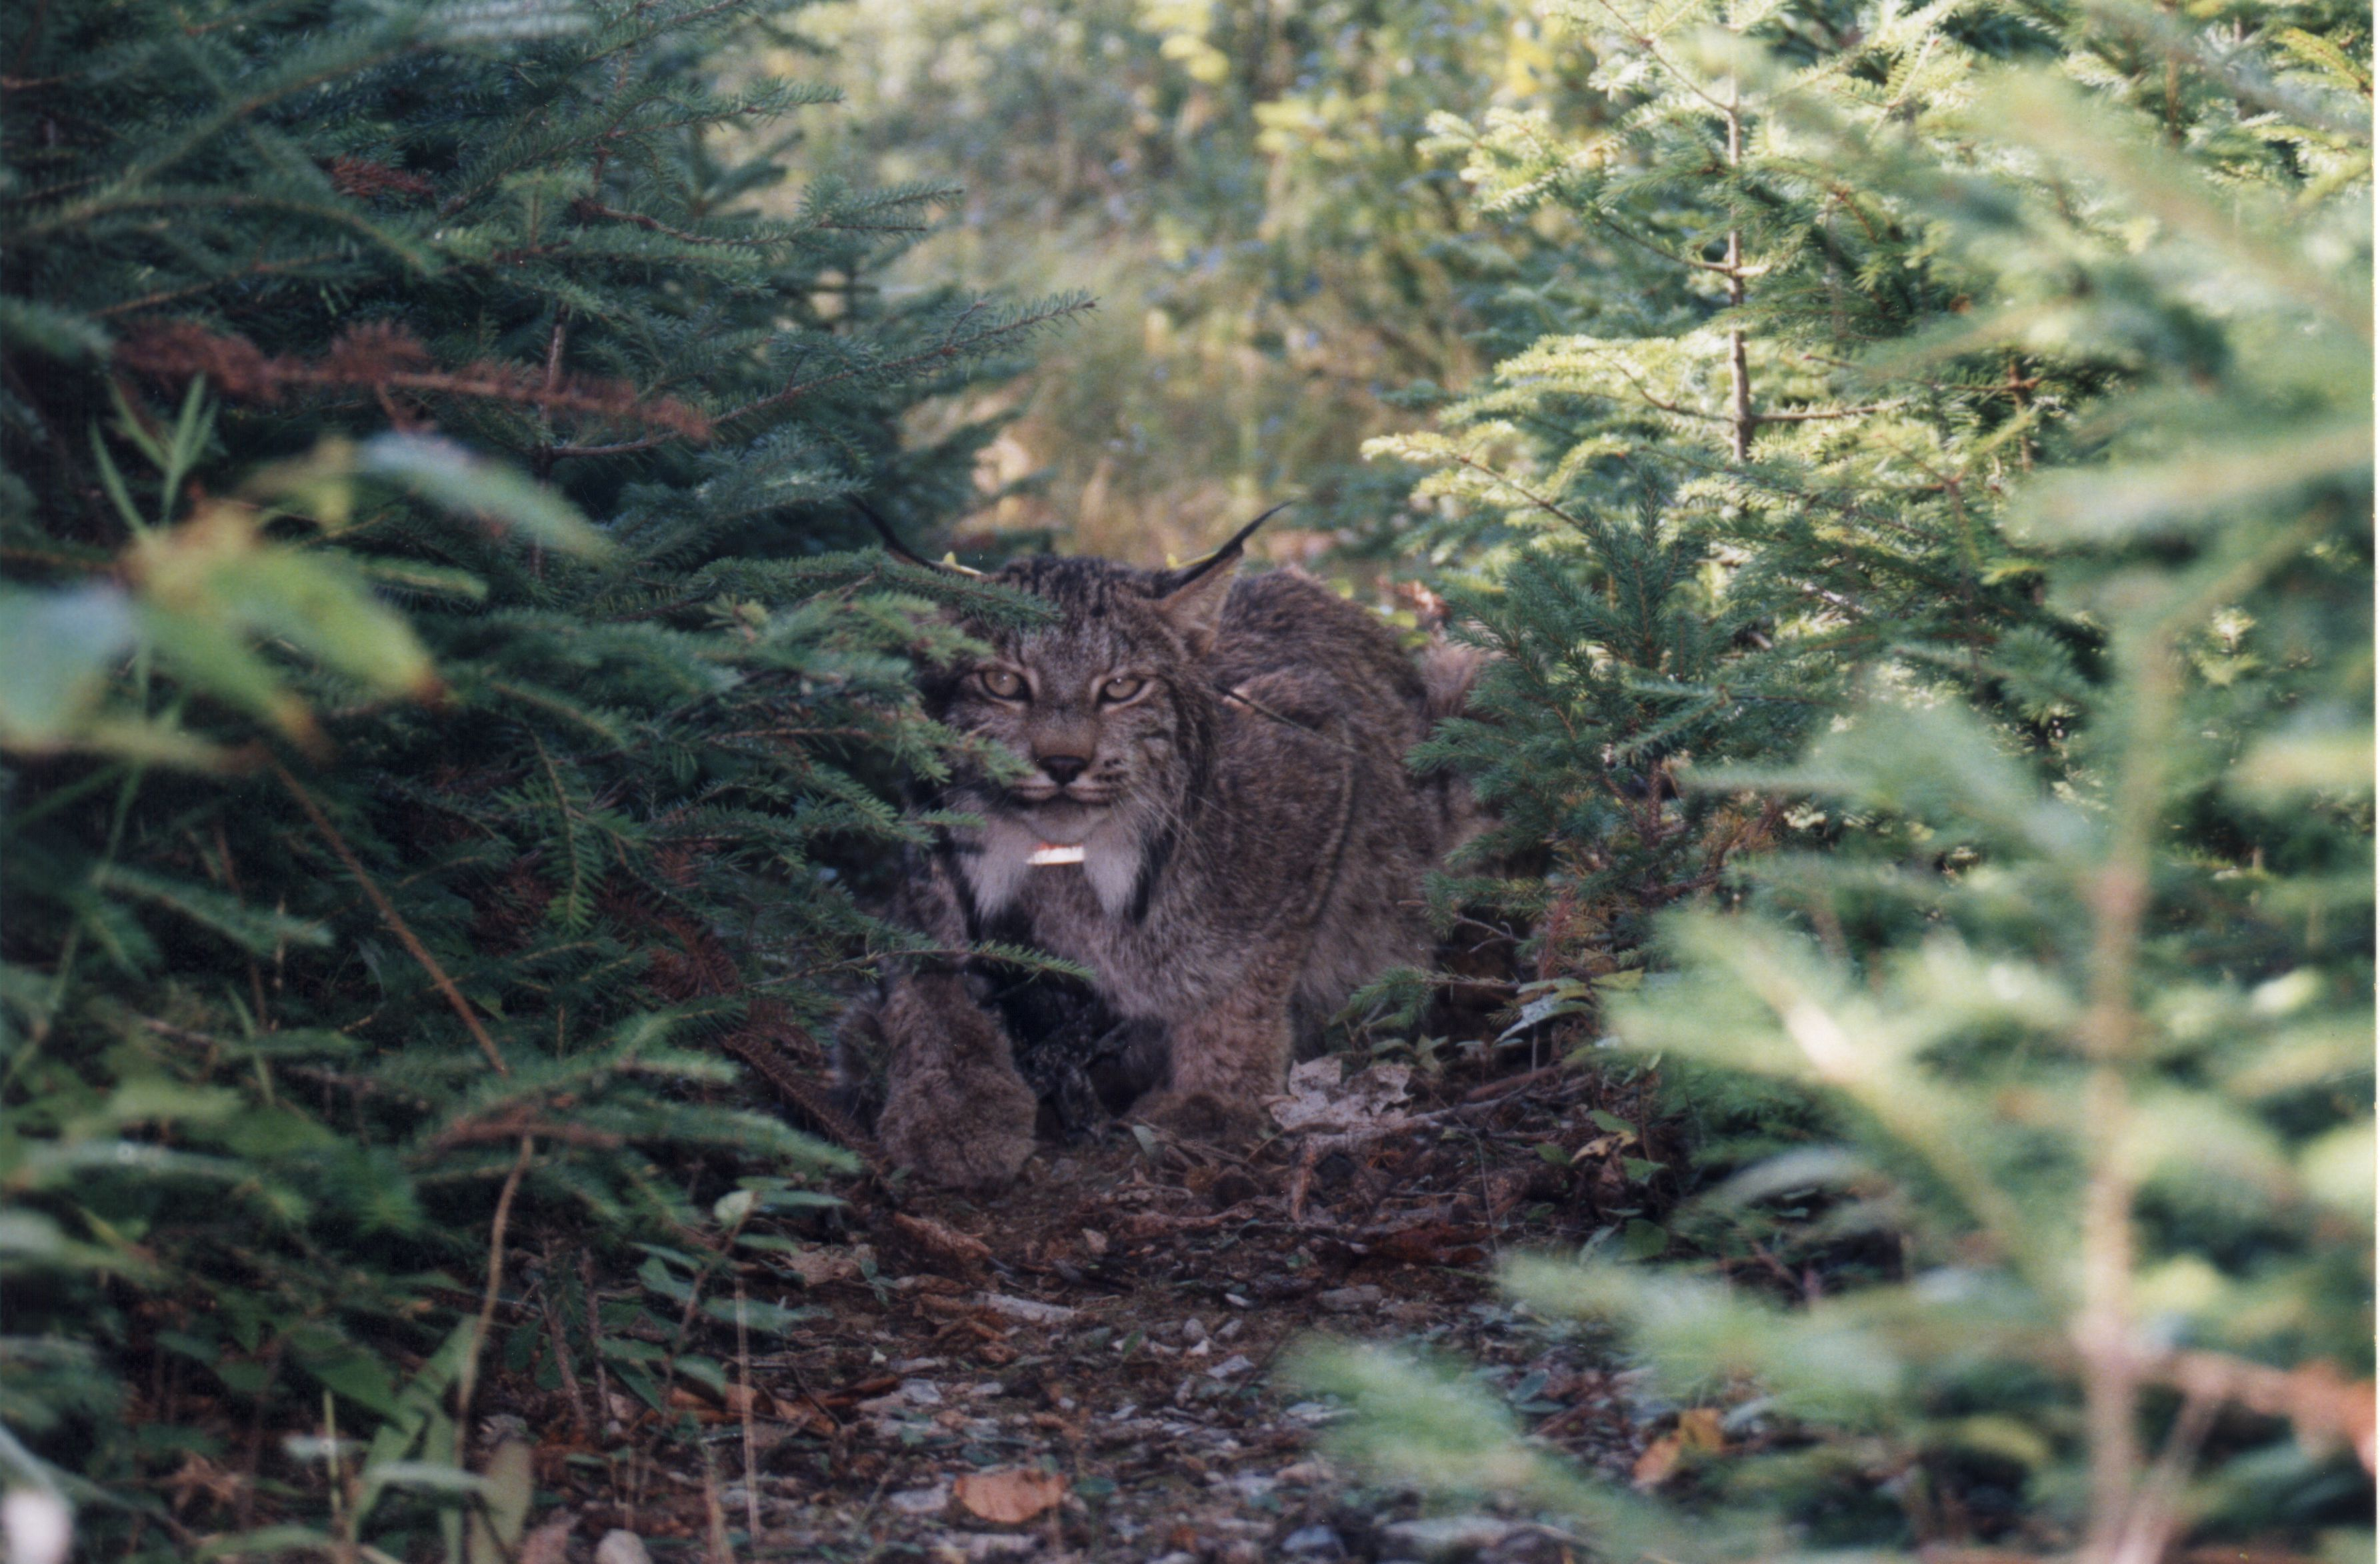
\includegraphics[width=\textwidth]{Ch20-Last/lynx.jpg}
\caption{
Canada Lynx, ear-tagged and radio collared, producing high quality
data in the name of science.
{\it Photo credit: A Fuller, Cornell University} }
\label{last.fig.lynx}
\end{figure}

You've finally made it to the last chapter and we realize it's been a
long journey to get here. Congratulations!  We hope this book has
provided you with many ideas on how to conduct ecological studies and
address specific questions that were previously thought difficult or
impossible to answer, and given you a solid foundation for carrying
out SCR analyses using either Bayesian or classical methods of
statistical inference.  However, we believe this journey is only just
beginning, and we leave you now with a few thoughts on what we see as
the future of SCR methods.

Let us first briefly consider how we got here. Over a century ago,
around 1786 in France, Pierre-Simon Laplace and others first developed
capture-recapture methods and introduced the study of populations
including spatially varying density. This was of course regarding
human population demography, but still, the foundation of how we would
go on to study animal populations was being laid out then and there.
The Lincoln-Petersen method was articulated by the 1930s and
development of capture-recapture models began to grow rapidly starting
in the 1950s.  Soon, capture-recapture methods had become a
cornerstone of ecological and wildlife modeling and analysis. Today,
spurred on by the advent and rapid development of non-invasive
technologies like DNA sampling, camera trapping, acoustic sampling,
and other methods, capture-recapture is more relevant and widely used
than ever before. These new survey methods allow researchers to use
capture-recapture for species that could not be studied efficiently
even a few years ago, especially those that are difficult to capture
or handle including most felids (Fig. \ref{last.fig.lynx}), bears,
mustelids such as fishers ({\it Martes pennanti},
Fig. \ref{last.fig.fisher}) or weasels (e.g., long-tailed weasel {\it
  Mustela frenata}, Fig. \ref{last.fig.weasels}), and many other
species.

With these new sampling techniques, like many commonly used
capture-recapture sampling methods, spatial information about location
of capture is collected.  Classical capture-recapture models ignore
this information, and in doing so fail to provide a formal method for
modeling spatial variation in density and encounter probability.  It
was these deficiencies that motivated the development of SCR models,
starting around 2003 - 2004.

We have seen a great increase in the number of papers that use or cite
SCR models, and to articulate and quantify this growth, we did a
Google Scholar search on March 6, 2013 using the terms:
\begin{small}
\begin{verbatim}
``spatial capture recapture'' OR ``spatially explicit capture recapture''
\end{verbatim}
\end{small}
The results from this literature search are shown in
Table~\ref{last.tab.cites}.  We see the number of citations involving
SCR rapidly increasing, with growth in citation counts after 2004
fueled by publication of \citet{efford:2004} and the release of the
software DENSITY \citep{efford_etal:2004}. In 2012 there were 84
articles published and 27 through the first 9 weeks of 2013.  The
results, we think, suggest a bright future for the development and
application of spatial capture-recapture models. Most (but not all) of
these papers are about the type of SCR models discussed in this book,
although a handful had to do with other types of spatial analysis as
related to capture-recapture models.

\begin{table}[ht]
\caption{Google Scholar citations by year based on a search of
{\tt ``spatial capture recapture'' OR ``spatially explicit
capture recapture''} conducted on March 6, 2013. The estimated growth
rate of this population of papers was 33.4\%.
}
\begin{tabular}{lcl} \hline \hline
Time period & Cumulative cites & Cites in year previous \\ \hline
since 2002 & 274 cites & \\
since 2003 & 274 cites &0 articles published in 2002 \\
since 2004 & 271 cites &3 articles published in 2003 \\
since 2005 & 269 cites &2 articles published in 2004 \\
since 2006 & 264 cites &5 articles published in 2005 \\
since 2007 & 261 cites &3 articles published in 2006 \\
since 2008 & 253 cites &8 articles published in 2007 \\
since 2009 & 242 cites &11 articles published in 2008 \\
since 2010 & 222 cites &20 articles published in 2009 \\
since 2011 & 176 cites &46 articles published in 2010 \\
since 2012 & 111 cites &65 articles published in 2011 \\
since 2013 & 27 cites &84 articles published in 2012 \\
& &27 published so far in 2013, since March 6
\\ \hline
\end{tabular}
\label{last.tab.cites}
\end{table}

We believe that use and growth of SCR modeling in conservation
biology, management, wildlife, fisheries, and many other disciplines
that we place under the general umbrella of ecology will only
continue.  This prediction is based our belief that SCR provides a
flexible framework for studying spatial and temporal variation in
ecological processes while acknowledging the fact that these processes
are almost always observed imperfectly.  The ``big idea'' of SCR, if
you could distill the whole thing into one idea, is based on extending
closed population models by augmenting them with a point process model
that describes the distribution of individuals \citep{efford:2004} in
space.  In a sense, that is really all there is to it.  It seems like
a little thing, a minor addition to a model, some incremental advance
or ``$\epsilon$-improvement'' of existing technology.  But the
relevance is much bigger and more profound because, once we have made
space explicit in the model, we can think about building population
models that embody explicit spatial processes and using those models
to improve our understanding of population biology and ecology, and to
test explicit hypotheses about mechanisms that govern populations.

We covered many ecological processes that can be studied using SCR,
such as landscape connectivity, resource selection, and spatial
variation in density. These are all by themselves profound extensions
of the basic capture-recapture method, and they broaden and expand the
relevance and utility of capture-recapture for studying animal
populations.  Although we filled almost 600 book pages (mostly) with
SCR methods, there remains much to be done in the continued
development of SCR models. In the following section, we highlight some
emerging topics that show promise or might be in need of further
development. Finally, we end with a few remaining thoughts on the use
of SCR models in the future.



\section{Emerging Topics}

In this book, we provided an overview and synthesis of
capture-recapture methods as known to us around the end of 2012. There
are many emerging topics which we have not covered either because of
lack of technical knowledge, lack of time for satisfactory
development, or lack of a good framework for implementation. Here we
present some of those topics. This is not a complete list by any
means, just a subset of topics that we or our colleagues are currently
working on, or that we think might make good PhD, Masters or other
research projects.


\subsection{Modeling territoriality}
\label{last.sec.ipp}

In currently developing work, \citet{reich_etal:2012} propose a model
that accounts for spatial variation in density and potential
interactions between individuals' territory centers.  Under this
model, the territory centers follow an inhomogeneous Strauss process
\citep{strauss:1975}, which includes a parameter that determines the
strength of repulsion between territory centers.  The idea is based on
the notion that territorial species would have well defined (and
defended) territories and thus activity centers may be more regular on
the landscape than predicted by a homogeneous point process.  A
simulation study demonstrated that properly accounting for
interactions between individuals can substantially improve population
size estimates in terms of bias and precision relative to the usual
independence model.

While the Strauss model is intuitive and shows great potential, it
presents computational challenges. The first challenge is that the
likelihood includes a high-dimensional integral that has no closed
form. To address this issue, \citet{reich_etal:2012} developed an
approximation to the Strauss likelihood which allows for posterior
sampling, extending related work for categorical Markov random fields
\citep{green_richardson:2002,smith_smith:2006}. The second challenge
is that $N$ is treated as an unknown parameter to be updated and hence
$N$ varies and so does the dimension of the posterior distribution.
In this case, the dimension-changing problem can be overcome by using
data augmentation, as we have done in many situations in this book.

\subsection{Combining data from different surveys}

In some instances, researchers apply different survey techniques to
the population of interest, because they yield complementary
information. For example, camera trapping is the prime tool for
estimating population size/density and other demographic parameters
for uniquely marked species, while genetic surveys can yield
additional information on the genetic diversity and health of a
population that cannot be studied using camera traps. At the same
time, genetic surveys, when samples are analyzed to the individual
level, also yield spatial capture recapture data (see
Chapt. \ref{chapt.search-encounter}). In this situation, we have two
data sets at hand that carry information on animal density, and we
should be able to get more precise estimates of density if we combine
these two data sets into a single SCR model.

\citet{gopalaswamy_etal:2012mee} developed two approaches to combining
data from different survey types. In the first case, both surveys are
carried out at the same time, so that we can assume that they both
sample the same -- closed -- animal population, i.e., there are no
possible changes in population density between the two surveys. For
camera trapping and genetic surveys, we cannot match records of
individuals between the two data sets. However, models for the
distinct sample methods may share some parameters (e.g., $\sigma$ of
the encounter probability model) and, if the studies were conducted
simultaneously, they share a common population size $N$.

A second approach of using information from one survey in the analysis
of a second survey (that maybe does not yield quite as much data as
the primary survey) is by analyzing the %your
primary data set alone, then
taking the posterior distribution of a parameter both surveys share
and using it as an informative prior distribution in the analysis of
the second data set. \citet{gopalaswamy_etal:2012mee} refer to this as
the stepwise approach, and they implemented this approach by equating
the mean and variance of the posterior distribution of $\psi$ and
$\sigma$ from the photographic survey to the mean and variance of a
beta and a gamma prior for these parameters, respectively, for the
genetic survey. The authors found that this approach produced almost
identical density estimates compared to the combined model approach
described above.

In summary, no matter which approach is chosen, combining data across
surveys can help researchers %to
obtain more precise population size or density estimates, which is
especially valuable when dealing with rare and elusive species like
big cats that almost always will produce sparse individual data sets.
The paper by \citet{gopalaswamy_etal:2012mee} considers the situation
where we have two SCR data sets, but we can imagine combining SCR data
with other sources of information, such as telemetry data (see
Chapt. \ref{chapt.partialID} and Chapt. \ref{chapt.rsf} for examples),
and possibly opportunistic observations, although to our knowledge
this latter issue has not been tackled in the context of SCR, yet.


\subsection{Misidentification}

Imperfect identification of individuals can happen in a variety of
ways. In genetic surveys there is usually some probability of
misidentification due to genotyping error
(e.g. \citet{lukacs_burnham:2005}). In camera trap survey a different
type of imperfect identification can occur when only the only one
flank of an animal is recorded in a detection event and cannot be
matched to any of the individuals identified by both flanks.
% XXX RC: Wait, do we mean "cannot be matched to other individuals
% identified by a just one flank"? If an animals is identified by both
% flanks, then a picture of just 1 side should be good enough right?
% XX RS: yeah, that's why the problem is when you get only one flank that's not in your both-flank sample
In that case, we can match single-flank pictures with the same side
flank pictures, but not with opposite side flank pictures and thus
cannot construct definite encounter histories for these single-flank
individuals (a right flank and a left flank picture could be the same
individual, or could be from two distinct individuals). Finally, in
Chapt. \ref{chapt.partialID}, in the context of mark-resight models,
we discussed the case where individuals can either not definitely be
identified as marked or not -- a violation of a basic mark-resight
assumption, and developed an approach to dealing with the situation
where we can always tell if an animal is marked or not, but we are not
always able to ascertain its individual identity.

In non-spatial capture recapture some efforts have been made to
formally deal with misidentification. \citet{stevick_etal:2001}
address this problem by double-sampling to derive an error rate for
genetic identification, and then including this error rate as a known
constant into a Lincoln-Petersen estimator of
abundance. \citet{lukacs_burnham:2005} develop an approach that
includes an additional parameter in the model -- the probability of a
genotype being identified correctly, which is estimated as part of the
model likelihood. \citet{link_etal:2010} developed an approach toward
solving the same problem implemented in a Bayesian framework that
relaxes some of the assumptions of the initial approach.
\citet{yoshizaki_etal:2009} deal with misidentification from camera
trap pictures due to evolving marks (i.e., natural marks that change
over time, such as scars). This situation is different from the
genotyping error one. Here, a change in marks creates a supposedly
`new' individual that can be recaptured several times, while the
original individual is never captured again (its mark is no longer in
the population). In contrast, in genotyping error it is assumed that
misidentification creates a `new' individual that is never observed
again, because each error leads to a new unique
genotype. \citet{yoshizaki_etal:2009} approach this situation
similarly, by including a parameter describing the probability of
correctly identifying an individual upon recapture (the parameter can
also be interpreted as the probability that a mark does not change
between capture occasions). Because of the dependencies between true
and false detection histories (when a `new' individual is created, the
`real' one can no longer be recaptured), the standard multinomial
approach to coming up with a model likelihood does not work and
implementing the model in a maximum likelihood framework is
difficult. The authors instead demonstrate an implementation of the
model based on minimizing a function of the squared differences
between the observed and expected frequencies of the observed capture
histories.

To our knowledge no attempts have been made to deal with
misidentification in an SCR framework. While all of the mis-ID cases
described above require distinct approaches, we believe that there is
one unifying theme to all of them: the capture locations of the %un or
potentially mis-identified records should be informative about
identity.  For example, a right flank and a left flank camera trap
picture that are taken at two neighboring camera traps should be %are
more likely to belong to the same individual that a right and a left
flank picture taken at cameras located at opposing ends of the trap
array, especially if animal movement is smaller than the extent of the
trap array.  SCR models provide a natural way of using this additional
information to reduce the uncertainty arising from misidentification.

\begin{comment}
\subsection{Three dimensional space}

Throughout this book we have treated space as two-dimensional, meaning
that activity centers are assumed to occur on the real plane. This
approximation of reality is reasonable for many terrestrial species,
but aquatic organisms, especially marine animals move about in
three-dimensional space. Treating space as three-dimensional could
also conceivably be useful in studies of flying organisms, or species
that use multiple strata of tall forests; however, we suspect that
two-dimensional models of space should suffice in such
contexts. Regardless, a three-dimensional view of space requires that
activity centers ${\bf s}_i$ are indexed by $x,y,z$ coordinates. In
theory, this presents no problem whatsoever. In practice, estimation
based on integrated likelihood methods must involve a
three-dimensional integration. This will clearly be more
computationally demanding, but it should be possible using packages
such as {\tt R2Cuba}.
\end{comment}

\subsection{Gregarious species}

One of the key assumptions of the SCR models that we described
throughout this book is that the activity centers are independent of
one another, but this assumption will be violated for species that
associate in pairs, family groups, or any other type of aggregation.
However, we believe that general models can be developed for use in
studies of gregarious species.

The two issues that must be addressed are that (1) detections are not
independent -- a trap that catches one individual of given group is
likely to capture others in the same group, and (2) the activity
centers ${\bf s}_{i}$ should appear clustered or, in fact, completely
redundant in some cases. A possible way to account for this is to
change our definition of ${\bf s}_i$ from the location of an
individual's activity center, to the location of a group's activity
center \citep{russell_etal:2012}. Ideally, to accommodate unknown
group size, the SCR model would be expanded to include a model
component for group size, so that formal estimation of both group
density and group size would be possible.



\subsection{Single Catch Traps}

In Chapt. \ref{chapt.poisson-mn} we covered multinomial models in
which an individual's probability of being captured in a trap is
independent of all other individuals.  This is the multi-catch type of
device in which traps never fill-up, but an individual can only be
caught in one trap in any given occasion. We suggested (following
\citet{efford_etal:2009euring}) that the multi-catch independent
multinomial model could be used for ``single catch'' traps (traps that
hold a single individual or ``fill up'') and that bias associated with
mis-specifying the model would be low under certain conditions (i.e.,
when the proportion of occupied traps is low).

As discussed in Chapt. \ref{chapt.poisson-mn},
Sec. \label{poisson-mn.sec.singlecatch}, we recognize that the {\it
  time}, or order, of capture of an individual in any trapping
interval will affect the encounter probability of subsequently
captured individuals. Thus if the order of capture was known, then
this information could be used to write the likelihood of the
detection model exactly. In practice, the order of capture is almost
never known, but it should be possible to regard capture order as a
latent variable and consider all possible orderings.  This would be
computationally intense and so we are working on a solution that
selects an arbitrary ordering of the captures as a practical
approximation to the single-catch process. This will hopefully lead to
a formal model for the the single catch trap problem.

\subsection{Model Fit and Selection}

Evaluation of model adequacy or ``fit'' is an important part of any
applied analysis. In Chapt. \ref{chapt.gof}, we offered up a number of
ideas based on standard considerations and adapted and applied them to
SCR models. However, these ideas have not been widely applied, or
evaluated, and much work needs to be done. In particular, some basic
analysis of their power under meaningful alternatives would increase
their relevance and possibly lead to insights for devising better
methods. This applies to both Bayesian and likelihood-based methods,
for which there are even fewer published applications of
goodness-of-fit assessment.

Similarly, we discussed model selection strategies using more-or-less
conventional ideas based on AIC/DIC, and model indicator variables
using the \citet{kuo_mallick:1998} method. Calibration of these
methods under alternatives is needed, along with some analysis of
sensitivity to density estimates to misspecification of certain model
components.



\subsection{Explicit movement models}


We briefly discussed the topics of dispersal, transience, and
migration in Chapts. \ref{chapt.searchencounter} and \ref{chapt.open}
and sketched out a few ideas that allow for dynamics related to
movement or migration.  Temporary emigration and transiency are two
topics where a significant amount of work has been accomplished in
non-spatial closed and open capture-recapture models
\citep{kendall_etal:1997, pradel_hines:1997, hines_etal:2003,
  clavel_etal:2008, gilroy_etal:2012,chandler_etal:2011}.
Additionally, models for dispersal (e.g., \citet{clobert_etal:2001,
  ovaskainen:2004, ovaskainen_etal:2008} and and other forms of
movement (e.g., \cite{jonsen_etal:2005, johnson_etal:2008b,
  mcclintock_etal:2012}) have received quite a bit of attention and
development in ecology.

With the recent development of SCR models, the framework is in place
to provide a formal integration of the movement dynamics governing the
processes of dispersal, emigration, and transiency.  Further, the
availability of SCR models that allow for explicit population dynamics
(survival, recruitment) \citep{gardner_etal:2010ecol} now sets the
stage to integrate models of movement dynamics directly with models of
population demography, and parameterize interactions among population
processes. What remains as an area of fruitful research is the
development of realistic models of movement dynamics, dispersal,
temporary emigration, and transiency that can be effectively fitted
given typical sparse individual encounter history data generated from
capture-recapture studies.  Dispersal and emigration can also be
related to the life stage of an individual in a certain population.
Ultimately, combining multi-state models where the states are age
classes or breeding status categories, with open population SCR models
and explicitly modeling patterns of movement and dispersal as a
function of state (e.g., age or size class) seems like an important
area of development.


\section{Final Remarks}

Everything in ecology is spatial, and now so too are capture-recapture
models, models which have been the cornerstone of ecological research
on populations for decades.  Historically, the main use of
capture-recapture was to obtain population size estimates, but SCR
models move the problem from one of estimation to one of formalizing
hypotheses about spatial and temporal variation in ecological
processes.  These processes include resource selection, landscape
connectivity, and how individuals organize themselves in space. SCR
models allow for this formalization by borrowing methods from spatial
statistics, but unlike many spatial models, SCR models include key
demographic parameters such as density and survival and thus allow for
mechanistic rather than just phenomenological descriptions of natural
variation.  For these reasons, we believe SCR models will continue to
be developed and extended, and their use will continue to grow.

However, much work still needs to be done to improve computational
feasibility, to address many technical or methodological holes in the
literature, and to make these methods more accessible to
practitioners.  We look forward to these developments and hope that
this book will help catalyze further exploration on this nascent
odyssey.













